\section{Case Studies}
\label{sec:cases}

SEAL is demonstrated on five longitudinal datasets from different domains. Four are public, and they are chosen because their driving structure is independently documented, so the discovered rules can be checked against an external account. They cover carbon dioxide emissions, pandemic mortality, national income, and air quality. The fifth is a large panel of Indian household finances, and it receives the fullest treatment, both because it motivated the method and because its target is a ratio for which the non-circularity discipline of Section~\ref{sec:algorithm} is required. Across the four public panels the outcome is consistent, in that the rules select the groups a domain account would predict although that account never enters the method, and the household panel then applies the same machinery to a question of policy interest. Table~\ref{tab:datasets} summarises the five panels, and the data preparation for each is described in Section~\ref{sec:data} before the results are discussed.

\begin{table}[t]
\centering
\small
\begin{tabular}{lllrrrr}
\toprule
Dataset & Entity & Target & $N$ & $T$ & Groups & Ratio \\
\midrule
CO2 & country & CO2 per capita & 208 & 33 & 5 & 0.44 \\
COVID & country & weekly deaths per million & 224 & 104 & 5 & 0.66 \\
World Bank & country & GDP per capita & 190 & 34 & 3 & 0.62 \\
EPA & monitoring site & PM2.5 & 526 & 180 & 4 & 0.75 \\
CMIE (health) & household & health spending share & 14652 & 90 & 3 & 0.87 \\
\bottomrule
\end{tabular}
\caption{The five longitudinal panels. $N$ is the number of entities, $T$ the number of time points, Groups the number of discovered subgroups including the default group, and Ratio the within-group distance ratio of the reported segmentation, where a smaller value means tighter trajectories.}
\label{tab:datasets}
\end{table}

The data preparation and the shared method configuration are given in Section~\ref{sec:data}. Figure~\ref{fig:cases} shows the discovered subgroups as mean trajectories for the four public panels, Table~\ref{tab:rules} states the rule that names each subgroup, and the subsections that follow read them in turn.

\begin{figure}[t]
\centering
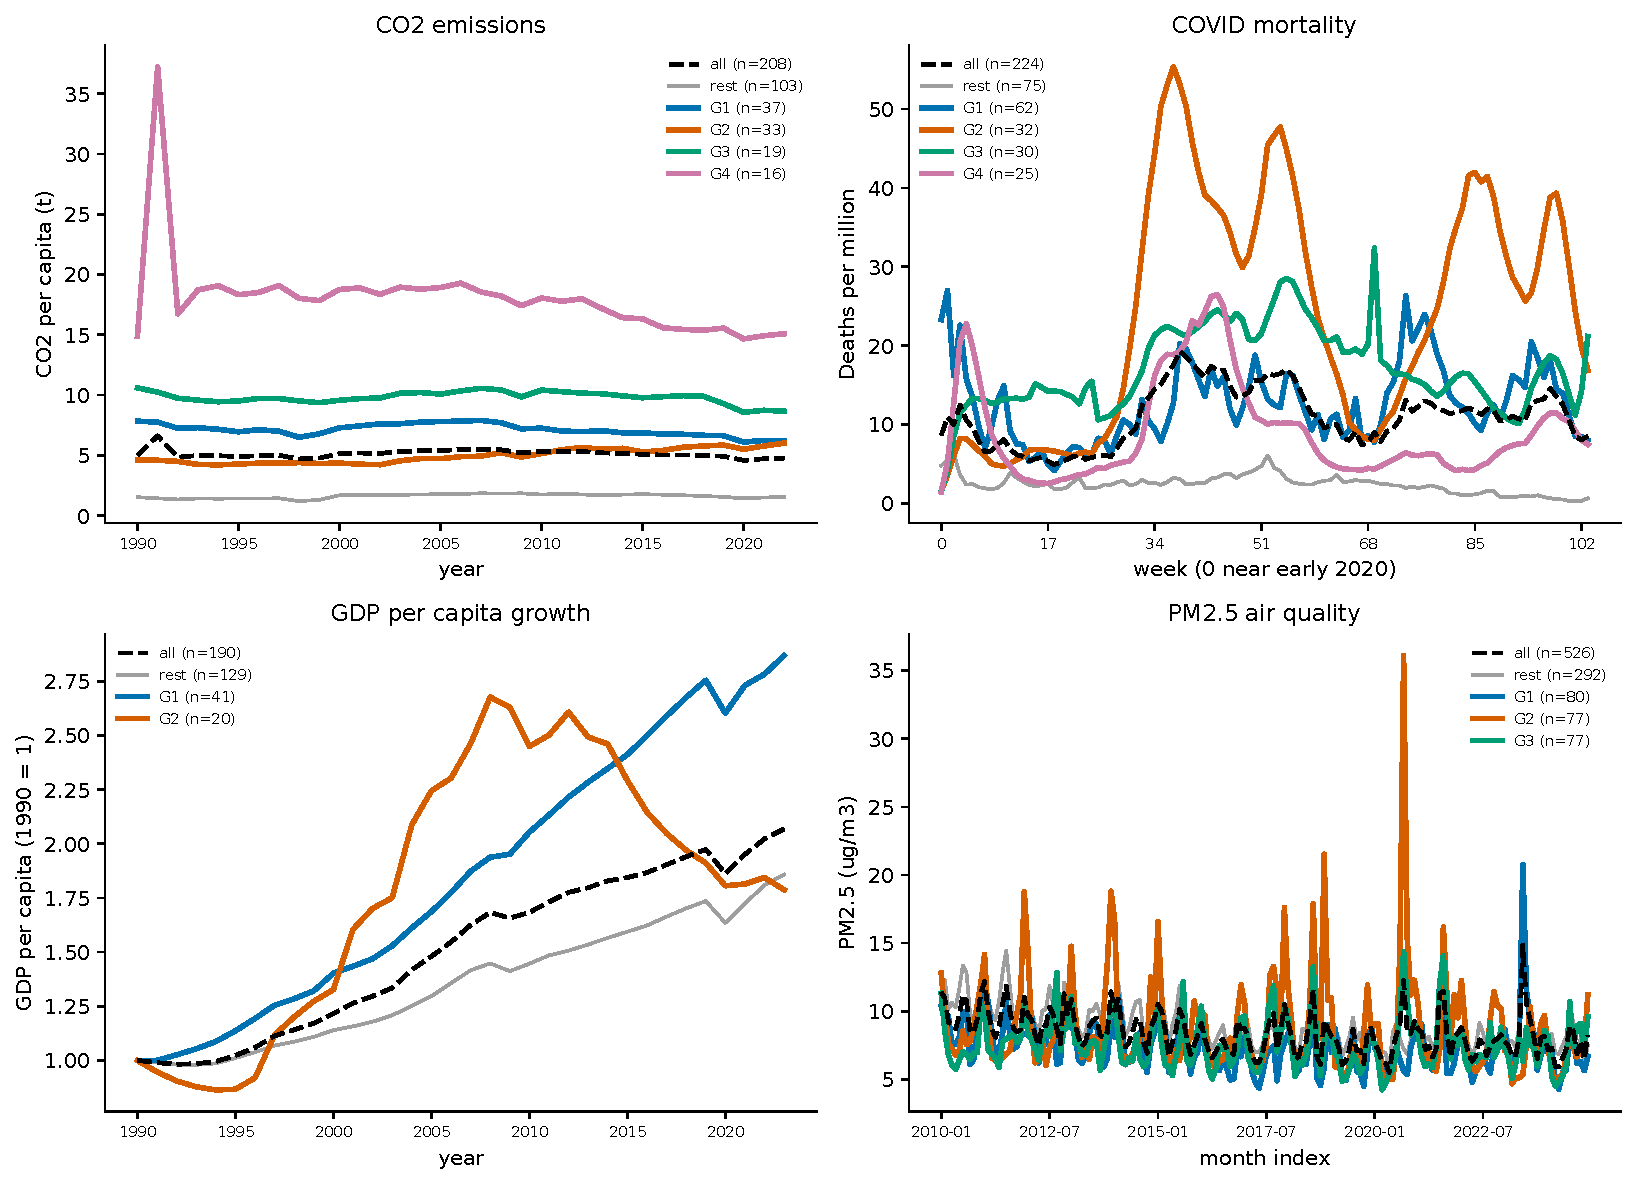
\includegraphics[width=\textwidth]{fig_case_trajectories.pdf}
\caption{Discovered subgroups on the four public panels, shown as the mean target trajectory of each group. The dashed black line is the population mean, the grey line is the leftover default group, and the coloured lines are the discovered subgroups with their sizes. Groups are numbered by size. In every panel the subgroups separate into distinct trajectory shapes that a rule then names.}
\label{fig:cases}
\end{figure}

\begin{table}[t]
\centering
\small
\renewcommand{\arraystretch}{1.2}
\begin{tabular}{@{}l r p{9.2cm}@{}}
\toprule
Panel & $n$ & Rule that defines the subgroup \\
\midrule
\multirow{4}{*}{CO2}
 & 16 & high income, gas-heavy fuel mix, little coal \\
 & 19 & high income, coal-heavy fuel mix \\
 & 37 & high income, little coal and little gas \\
 & 33 & upper-middle income, large population, low oil share \\
\midrule
\multirow{4}{*}{COVID}
 & 62 & older population, small country \\
 & 32 & older population, mid-size and sparse \\
 & 30 & older population, very large and sparse \\
 & 25 & older population, mid-size and dense \\
\midrule
\multirow{2}{*}{World Bank}
 & 41 & birth rate low and still falling \\
 & 20 & birth rate high, access to electricity flat \\
\midrule
\multirow{3}{*}{EPA}
 & 77 & longitude at most $-118^\circ$, the western sites \\
 & 77 & longitude between $-118^\circ$ and $-100^\circ$ \\
 & 80 & longitude above $-100^\circ$ and latitude above $42^\circ$ \\
\midrule
\multirow{2}{*}{CMIE (health)}
 & 2389 & eldest member over 60, low consumption borrowing \\
 & 3462 & high propensity to borrow for consumption \\
\bottomrule
\end{tabular}
\caption{The rule that defines each discovered subgroup, stated in plain terms with rounded thresholds. Each panel also has a default group, not listed, that collects the entities no rule selects. The exact machine-readable thresholds are given in the text of each case study. For the household panel the rules describe cohorts by attribute and never identify an individual household.}
\label{tab:rules}
\end{table}

\subsection{Are the subgroups exceptional?}
\label{sec:validation}

Before reading the rules of each panel, we ask whether the discovered subgroups are exceptional in a measurable sense, or whether a grouping this coherent could arise by chance. Two tests answer this, and Table~\ref{tab:validation} collects the numbers.

The first is a coherence test. The within-group distance ratio measures how tight the grouped trajectories are relative to the population, and a smaller value means tighter groups. To calibrate it we hold the group sizes fixed and permute the labels across entities two thousand times, which yields the ratio a random grouping of the same shape would reach. A random grouping sits near one, as expected, whereas the discovered grouping falls far below it in every panel, by between three and thirteen standard deviations of the permutation distribution, with an empirical $p$ below $0.001$ throughout. The rule-induced partition therefore captures trajectory structure that random assignment does not recover.

The second is an outcome-stratification test. The rules are built on descriptors and never on the target, so the groups differing on the target is not automatic. A Kruskal-Wallis comparison of each entity's mean target level across the discovered groups rejects the null of equal distributions in every panel, at $p$ below $10^{-6}$, which shows that the descriptor rules stratify the outcome rather than some incidental attribute. The separation is sharpest for the extreme groups. The highest-emitting carbon group stands almost two population standard deviations above the mean, and the highest-mortality COVID group stands more than one above it. Where the target is a growth index rather than a level, as for national income, the level-based effect size is small by construction, because those groups differ in the shape of their growth rather than in its height, and there the coherence test, which compares whole cumulative trajectories, carries the evidence.

\begin{table}[t]
\centering
\small
\begin{tabular}{@{}l r r r r@{}}
\toprule
Panel & ratio $r$ & random $r$ & $z$ & Kruskal-Wallis $H$ \\
\midrule
CO2        & 0.44 & 1.00 & 8.8  & 134 \\
COVID      & 0.66 & 1.00 & 13.1 & 112 \\
World Bank & 0.62 & 1.00 & 3.2  & 27 \\
EPA        & 0.75 & 1.00 & 12.0 & 76 \\
\bottomrule
\end{tabular}
\caption{Evidence that the discovered subgroups are exceptional. The observed within-group distance ratio $r$ is far below the ratio a size-matched random grouping reaches, by $z$ standard deviations of a two-thousand-fold permutation (all $p < 0.001$). The Kruskal-Wallis statistic tests whether the groups differ on the target itself, and it is significant in every panel at $p < 10^{-6}$ even though the rules never see the target.}
\label{tab:validation}
\end{table}

Finally, we ask whether the engineered temporal descriptors of Section~\ref{sec:temporal} earn their place. We rerun the identical search with a point-in-time snapshot, in which each numeric covariate contributes only its last observed value rather than its trend and its shortfall history, and we compare the best distance ratio. The answer depends on the domain, and the pattern is itself informative (Table~\ref{tab:ablation}). For national income the temporal features lower the ratio markedly, from $0.69$ to $0.62$, and they do so with a slightly shorter rule, because the group that matters is defined by a birth rate that is still falling, a movement a snapshot cannot see. For carbon emissions the two descriptor sets tie, because the emitting groups are set by income and fuel levels that the snapshot already carries. For mortality and for air quality the snapshot is marginally tighter, because those targets track a recent level rather than a movement, so the additional temporal columns only widen the search. Temporal features therefore help when the trajectory structure turns on how a covariate moved rather than on where it stands, and the income study is the clearest such case. The main runs use the temporal descriptors throughout for a single comparable protocol, at the cost of a little tightness on the panels that do not need them.

\begin{table}[t]
\centering
\small
\begin{tabular}{@{}l r r r@{}}
\toprule
Panel & snapshot $r$ & temporal $r$ & change \\
\midrule
CO2        & 0.44 & 0.44 & $0.00$ \\
World Bank & 0.69 & 0.62 & $-0.06$ \\
COVID      & 0.62 & 0.66 & $+0.04$ \\
EPA        & 0.75 & 0.75 & $+0.00$ \\
\bottomrule
\end{tabular}
\caption{Feature-engineering ablation. The best within-group distance ratio under a point-in-time snapshot of the covariates against the full engineered temporal features, with the search held identical. A negative change means the temporal features give tighter groups. They help most for national income, whose defining group is set by a falling birth rate, and are neutral or slightly costly where the target tracks a recent level rather than a movement.}
\label{tab:ablation}
\end{table}

\subsection{Carbon dioxide emissions}
\label{sec:co2}

The entities are 208 countries observed yearly from 1990 to 2022, and the target is carbon dioxide emitted per person. The covariates are national income per capita, population, and the shares of coal, oil, and gas in the energy mix, each turned into temporal features.

The reported segmentation reaches a distance ratio of $0.44$, the tightest of the five panels, so grouped countries are markedly closer in their emission paths than two countries picked at random. The rules read almost entirely off income level and fuel mix, and the groups they carve out are easy to recognise. The highest-emitting group, close to eighteen tonnes per person, is selected by high income together with a large gas share and a small coal share, and it holds the Gulf producers such as Qatar, Kuwait, the United Arab Emirates, and Saudi Arabia alongside the United States and Canada. A second wealthy group is selected instead by a large coal share, and it holds the coal-reliant industrial economies such as Russia, Germany, Poland, Australia, and Kazakhstan. A third wealthy group carries neither much coal nor much gas and sits lower, holding countries such as Luxembourg, Ireland, and Denmark whose electricity leans on nuclear power or renewables. A separate group of middle-income producers such as South Africa, Iran, and Belarus sits lower still, and the large default group collects the developing countries whose per-capita emissions stay low. Emission trajectories are thus organised first by how rich a country is and then by what it burns, which matches the standard account of emissions although that account is never supplied to the method. Each stratum arrives already named by a rule, so one can point to the coal-reliant wealthy group or the gas-rich group rather than merely note that a cluster exists.

\subsection{COVID-19 mortality}
\label{sec:covid}

The entities are 224 countries observed weekly across roughly two years from the start of the pandemic, and the target is reported deaths per million. The covariates are national attributes that stay fixed over the window, such as median age, population, population density, income, diabetes prevalence, hospital beds, and life expectancy.

The first and strongest split is on median age. Countries with an older population form the subgroups that carry the higher mortality trajectories, while the default group collects younger-population countries such as Bolivia, Namibia, and Guatemala whose recorded mortality stays lower. Among the older-population countries the further splits are on population size and density, and the groups they produce are geographically coherent even though geography was never a descriptor. One group holds the Western European countries such as the United Kingdom, Italy, Belgium, and Germany, which took a sharp early peak in the spring of 2020. Another holds the Eastern European countries such as Bulgaria, Hungary, Czechia, and Slovakia, which carried the highest sustained mortality across the later waves. A third holds the large countries of the Americas together with Russia, such as Peru, Brazil, the United States, and Argentina, whose mortality stayed high for a prolonged stretch. SEAL recovers the age-structure driver that dominated cross-country mortality and then separates the regional waves using nothing more than population size and density, and it states the split as a few readable conditions rather than as a regression coefficient. The distance ratio of $0.66$ is looser than for emissions, which is expected because weekly mortality is noisier and more affected by reporting differences than a slow annual quantity.

\subsection{Gross domestic product per capita}
\label{sec:worldbank}

The entities are 190 countries observed yearly from 1990 to 2023. The target is gross domestic product per capita expressed relative to its 1990 value, so every trajectory starts at one and its shape records the growth path since 1990. The covariates are demographic and infrastructure indicators, namely birth rate, death rate, access to electricity, internet use, and trade in services.

The segmentation separates countries by the shape of their growth path, and the rules key on demographic and infrastructure markers. One subgroup collects countries whose birth rate is low and still falling, and these follow the strongest sustained growth, rising to close to three times their 1990 level by the end of the window. It holds the Asian catch-up economies such as China, India, South Korea, Sri Lanka, Bhutan, and Vietnam, whose long climb is the clearest growth story of the period. A second subgroup collects countries whose birth rate is high and whose access to electricity stays essentially flat over the window, and these follow a rise-then-decline path, climbing through the commodity boom of the 2000s and then falling back toward their starting level. It holds the resource-dependent economies such as Equatorial Guinea, Chad, Nigeria, Iraq, and Niger, whose fortunes tracked the oil and mineral cycle. The remaining countries follow a moderate steady rise. Separating a boom-and-bust trajectory from a steadily rising one, even though both end above where they began, is what a shape-based grouping buys over a comparison of ending levels, and a high birth rate paired with stagnant electrification is a compact, testable signature of the resource-dependent group. The birth rate enters both through its level and through its trend, which is possible only because the descriptor set includes engineered temporal features rather than a single snapshot.

\subsection{Fine particulate air quality}
\label{sec:epa}

The entities are 526 air-quality monitoring sites in the United States observed monthly from 2010 to 2024, and the target is the concentration of fine particulate matter. The covariates include the coordinates and elevation of each site together with categorical descriptors of land use and setting, such as residential, industrial, or rural.

The categorical descriptors were available to the search as one-hot columns, yet the rules that separate the particulate trajectories key on geography, specifically bands of longitude together with latitude. One subgroup collects the western sites, and it turns out to be almost entirely Californian. Another collects the mountain and central-western band, holding sites in states such as Montana, Idaho, and Arizona. A third collects the northern sites of the upper Midwest around the Great Lakes, in states such as Michigan, Wisconsin, and Iowa. The large default group holds the eastern and southern sites, in states such as Pennsylvania, Ohio, Indiana, and Texas. Fine-particulate trajectories in the United States are thus organised more by region than by the recorded land-use label of the individual site. This is a useful negative result as much as a positive one. SEAL had the vocabulary to describe the subgroups by land use, since residential, industrial, and rural labels were all present as descriptors, and it did not use them, which says that the dominant structure over this period is spatial rather than local to the type of site. The looser distance ratio of $0.75$ reflects the strong seasonal cycle in the raw series, which every site shares and which therefore limits how tight any grouping can be.

\subsection{Household health spending}
\label{sec:cmie}

The setting that motivated this work is the burden that health spending places on household budgets. The entities are Indian households drawn from the Consumer Pyramids Household Survey collected by the Centre for Monitoring Indian Economy, and the target is the share of household income spent on health, measured monthly. Because the target is a ratio of health spending to income, the preparation and the descriptor rules described in Section~\ref{sec:algorithm} matter more here than anywhere else. The results in this subsection are reported at the level of subgroups and rules only, in keeping with the terms under which the data are held, and no household-level record is shown. The sample is not a population sample, so the findings describe the surveyed households rather than the country.

\paragraph{Target and window.} The target of a household in a month is the logarithm of one plus the ratio of health spending to income. Months whose income falls below the fifth percentile of positive income are dropped so that a near-zero denominator cannot manufacture an extreme share, and data-collection sentinels are removed while genuine zero-spending months are kept as signal. The analysis is placed on a fixed window of ninety months running from June 2016 to November 2023, which is centred on the onset of the pandemic in March 2020 so that an equal span of roughly three and a half years lies on either side of the shock. A household enters the cohort when it is observed across at least ninety percent of the window, and the few remaining internal gaps are filled by linear interpolation. This admits 14652 households, and the whole cohort is used with no sampling. Figure~\ref{fig:cmie_window} shows how panel coverage varies over the calendar and where the window sits.

\begin{figure}[t]
\centering
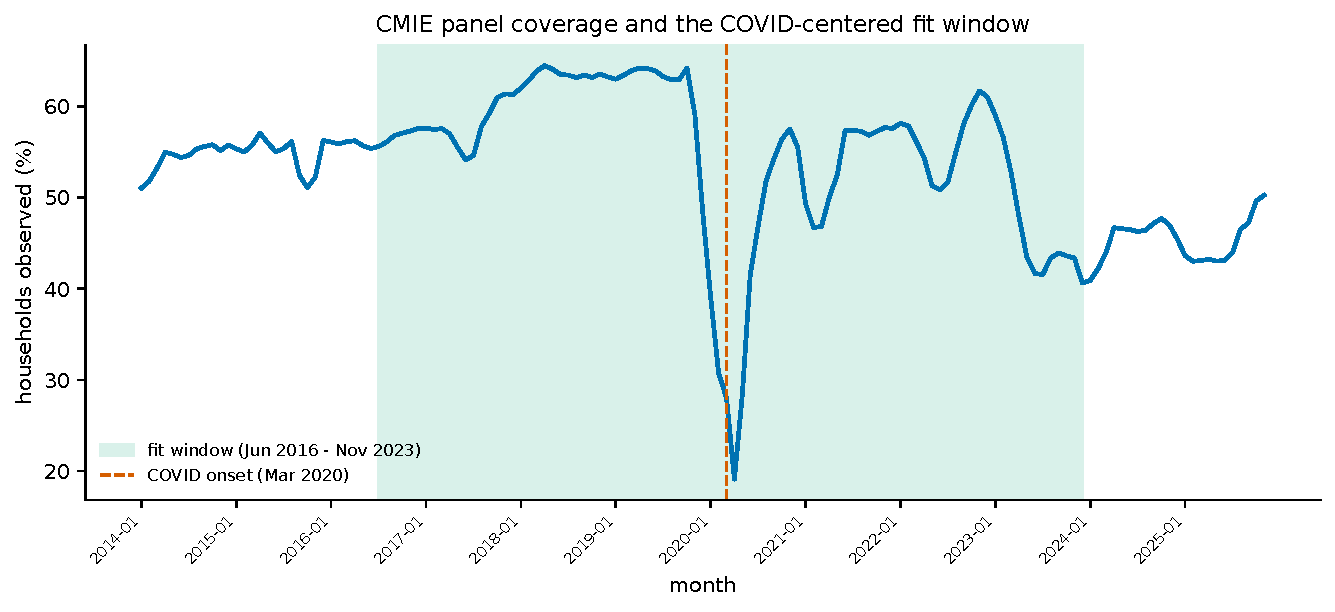
\includegraphics[width=0.82\textwidth]{fig_cmie_window.pdf}
\caption{Coverage of the household panel over the calendar, measured as the share of households observed in each month, together with the ninety-month fit window centred on the pandemic onset. The window is placed where enough households are observed continuously that complete trajectories can be required rather than imputed at scale.}
\label{fig:cmie_window}
\end{figure}

\paragraph{Descriptors and design choices.} The descriptors combine static household attributes with engineered temporal features of household income. Static attributes include household composition, education, occupation, insurance cover, and the propensity to borrow for non-medical purposes, with categorical attributes one-hot encoded. The income descriptors are computed over the same ninety-month window as the target, and they include the trend, the volatility, the largest single drop, the number of drops, the largest income falls in the pre-pandemic, pandemic, and recovery sub-windows, and the depth, length, and recency of the worst sustained income shortfall. The non-circularity rule is enforced strictly. Health-spending columns are forbidden as descriptors because they form the numerator of the target, and the income level is forbidden because it is the denominator, while income dynamics are retained because a statement about how income moved is not a restatement of the target.

\paragraph{Results.} The segmentation returns three subgroups over the 14652 households, and the reported rule set has a cost of $0.887$ with a within-group distance ratio of $0.872$. The default group holds 8801 households and carries the lowest health-spending burden. A first subgroup of 2389 households is selected by the condition that the oldest household member is above sixty and that consumption borrowing is low, and it carries the highest burden of the three. A second subgroup of 3462 households is selected by a high propensity to borrow for consumption, and it carries an elevated burden that sits between the other two. The burden of health spending thus concentrates in households with an elderly member and in households under financial stress, and the two conditions select largely different households, since the elderly rule is stated for households that are not already heavy consumption borrowers. Both conditions are structural or behavioural rather than mechanical, since neither the age of a member nor borrowing for consumption is the income denominator of the target, so the elevated burden reflects genuinely higher health spending rather than a shrinking denominator. Figure~\ref{fig:cmie_subgroups} shows the three mean trajectories.

\begin{figure}[t]
\centering
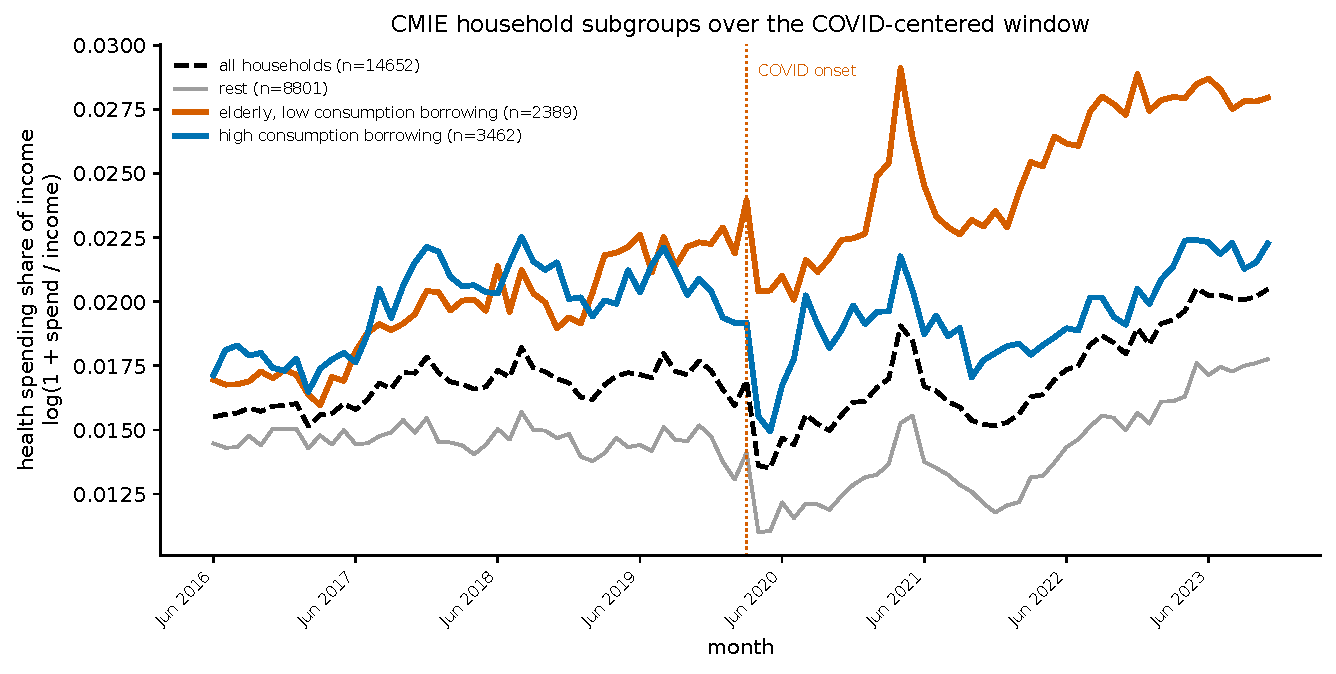
\includegraphics[width=0.85\textwidth]{fig_cmie_subgroups.pdf}
\caption{Health-spending burden for the three discovered household subgroups over the COVID-centered window. Households with an elderly member carry the highest burden and households that borrow heavily for consumption carry an elevated one, while the remaining households stay lower. All three trajectories dip sharply at the onset of the pandemic, when the lockdown cut off routine care, and then rebound.}
\label{fig:cmie_subgroups}
\end{figure}

Two features of the result deserve comment. The distance ratio of $0.872$ is high, which means that the subgroups are broad tendencies rather than tight clusters, so the rules identify where the burden concentrates without claiming that every household in a group traces the same path. The single best rule keys on age and on consumption borrowing rather than on the engineered income features, yet the engineered temporal features are far from idle. Across the diverse alternative rule sets they appear repeatedly, including the size of the income drop in the pre-pandemic and pandemic sub-windows and the severity of the worst sustained income shortfall, which shows that the temporal construction of Section~\ref{sec:temporal} supplies competitive descriptors even when the shortest rule does not need them. The trajectories in Figure~\ref{fig:cmie_subgroups} also carry a clear temporal signal that no rule was asked to find, namely a sharp fall in the burden at the onset of the pandemic followed by a rebound. This fall may look surprising, since a health shock might be expected to raise the burden rather than lower it, and it merits a careful reading. In the cohort the mean monthly health spending fell by about forty-nine percent between February and April 2020 while mean income fell by about forty-three percent over the same months, so the numerator of the burden fell faster than its denominator and the ratio dropped. The drop therefore records care that was not obtained rather than relief that was gained, because the lockdown closed clinics, halted transport, and deterred visits, and it suppressed routine and elective health spending more sharply than it suppressed income. Read this way a falling burden is an adverse signal of unmet need, and the rebound that follows is consistent with deferred care returning once the strictest restrictions lifted and with the pandemic waves themselves adding to health spending. The example shows why a ratio target has to be interpreted together with its parts, which is exactly what the non-circular treatment of income in Section~\ref{sec:temporal} was designed to keep visible.
